% Build from the repository root:
% mkdir -p .cache/figures
% pdflatex -halt-on-error -output-directory=.cache/figures docs/figures/code-structure.tex
% cp .cache/figures/code-structure.pdf docs/figures/
% pdftoppm -png -r 160 -singlefile docs/figures/code-structure.pdf docs/figures/code-structure
\documentclass[tikz,border=12pt]{standalone}
\usepackage[T1]{fontenc}
\usepackage{lmodern}
\usetikzlibrary{arrows.meta,calc}

\definecolor{ink}{HTML}{13263A}
\definecolor{muted}{HTML}{4A6075}
\definecolor{line}{HTML}{526B82}
\definecolor{border}{HTML}{B9CBDC}
\definecolor{modulefill}{HTML}{F2F7FC}
\definecolor{artifactfill}{HTML}{F2F8F6}
\definecolor{artifactborder}{HTML}{ADC9C2}
\definecolor{orchestrator}{HTML}{1C4464}

\newcommand{\cardtext}[2]{\textbf{\texttt{#1}}\\[3pt]#2}
\newcommand{\anglelabel}[1]{\textless#1\textgreater}

\begin{document}
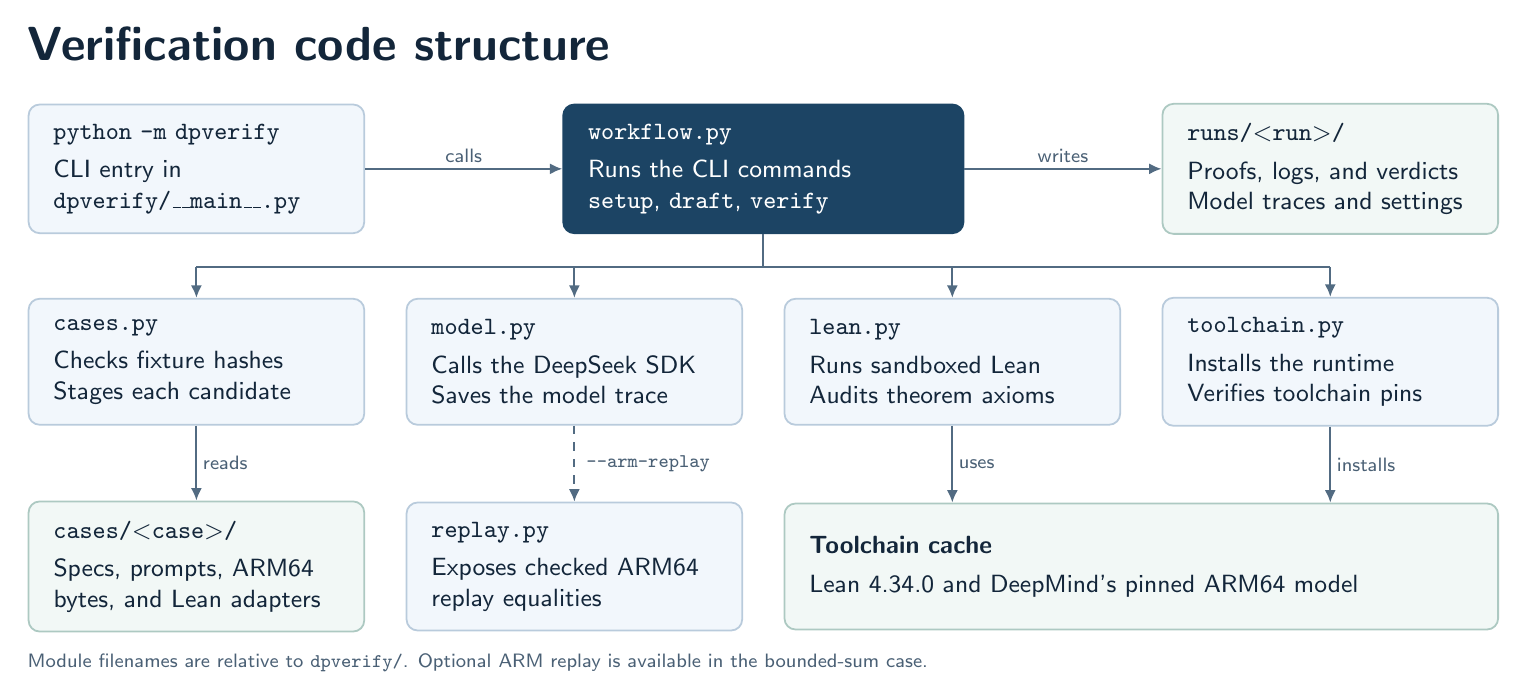
\begin{tikzpicture}[
  x=1cm,
  y=1cm,
  card/.style={
    rounded corners=4pt, inner xsep=9pt, inner ysep=7pt,
    align=left, text width=3.63cm, minimum height=1.60cm,
    font=\sffamily\small, text=ink, draw=border, fill=modulefill,
    line width=.65pt
  },
  core/.style={card, fill=orchestrator, draw=orchestrator, text=white},
  artifact/.style={card, fill=artifactfill, draw=artifactborder},
  connector/.style={draw=line, line width=.75pt},
  link/.style={connector, -{Latex[length=4.5pt,width=4pt]}},
  relation/.style={
    font=\sffamily\scriptsize, text=muted, fill=white, inner sep=2pt
  }
]
  \node[anchor=north west, inner sep=0pt, text=ink,
        font=\sffamily\bfseries\fontsize{19}{22}\selectfont]
        at (0.15,0) {Verification code structure};

  \node[card] (entry) at (2.3,-1.80)
        {\cardtext{python -m dpverify}{CLI entry in\\\texttt{dpverify/\_\_main\_\_.py}}};
  \node[core, text width=4.45cm] (workflow) at (9.5,-1.80)
        {\cardtext{workflow.py}{Runs the CLI commands\\\texttt{setup}, \texttt{draft}, \texttt{verify}}};
  \node[artifact] (runs) at (16.7,-1.80)
        {\cardtext{runs/\anglelabel{run}/}{Proofs, logs, and verdicts\\Model traces and settings}};

  \node[card] (cases) at (2.3,-4.25)
        {\cardtext{cases.py}{Checks fixture hashes\\Stages each candidate}};
  \node[card] (model) at (7.1,-4.25)
        {\cardtext{model.py}{Calls the DeepSeek SDK\\Saves the model trace}};
  \node[card] (lean) at (11.9,-4.25)
        {\cardtext{lean.py}{Runs sandboxed Lean\\Audits theorem axioms}};
  \node[card] (toolchain) at (16.7,-4.25)
        {\cardtext{toolchain.py}{Installs the runtime\\Verifies toolchain pins}};

  \node[artifact] (fixtures) at (2.3,-6.85)
        {\cardtext{cases/\anglelabel{case}/}{Specs, prompts, ARM64\\bytes, and Lean adapters}};
  \node[card] (replay) at (7.1,-6.85)
        {\cardtext{replay.py}{Exposes checked ARM64\\replay equalities}};
  \node[artifact, text width=8.43cm] (runtime) at (14.3,-6.85)
        {\textbf{Toolchain cache}\\[3pt]Lean 4.34.0 and DeepMind's pinned ARM64 model};

  \draw[link] (entry.east) -- node[relation, above] {calls} (workflow.west);
  \draw[link] (workflow.east) -- node[relation, above] {writes} (runs.west);

  \coordinate (bus) at (9.5,-3.05);
  \draw[connector] (workflow.south) -- (bus);
  \draw[connector] (cases.north |- bus) -- (toolchain.north |- bus);
  \foreach \module in {cases,model,lean,toolchain}
    \draw[link] (\module.north |- bus) -- (\module.north);

  \draw[link] (cases.south) -- node[relation, right] {reads} (fixtures.north);
  \draw[link, dashed] (model.south) --
        node[relation, right, xshift=2pt] {\texttt{-\kern0pt-arm-replay}} (replay.north);
  \draw[link] (lean.south) --
        node[relation, right] {uses} (lean.south |- runtime.north);
  \draw[link] (toolchain.south) --
        node[relation, right] {installs} (toolchain.south |- runtime.north);

  \node[anchor=north west, inner sep=0pt, text=muted, font=\sffamily\scriptsize]
        at (0.15,-7.95)
        {Module filenames are relative to \texttt{dpverify/}. Optional ARM replay is available in the bounded-sum case.};
\end{tikzpicture}
\end{document}
